\chapter{Estado del arte}

\section{Dominio del problema}

\subsection{Aplicaciones móviles}

Los ``smartphones'' o teléfonos inteligentes han cambiado el paradigma de acceso a internet. Desde sus primeras apariciones a principios de la década de 2010, el uso y expansión de sus dispositivos ha aumentado exponencialmente. La evolución de estos sistemas ha incurrido y convertido muchos modelos de negocio

Actualmente casi cualquier persona tiene un teléfono móvil, con la posibilidad de acceder a miles de aplicaciones desarrolladas para estos dispositivos. Actualemnte los móviles no solo cumplen una función de comunicación entre personas, si no que han abierto con su desarrollo un abanico de oportunidades.

Aunque el enfoque inicial de este tipos de dispositivos fuese el de ser una herramienta de comunicación, el avance tecnológico ha permitido que cada vez puedan ser usados como herramientas de trabajo. Pantallas cada vez más grandes y soluciones para convertir móviles en dispostivos de escritorio hacen que el desarrollo de aplicaciones móviles no se limite al propio dispositivo. 

Cabe destacar que cada vez más el desarrollo de aplicaciones móviles se está fusionando con el de soluciones de escritorio. Desde la aparición de frameworks como React Native o Flutter, hasta la aparición de ordenadores con CPU basados en la arquitectura ARM, hacen cada vez más fina la línea entre ambos dispositivos. 

Este enfoque es el que se quiso buscar a la hora de decidir la solución tecnológica buscada por la \textit{Fundación Escuela de Solidaridad}. Para ellos era importante, como se ha comentado previamente, la inmediatez en el acceso a la información. En la mayoría de las situaciones en las que necesitan consultar la información de los residentes, no tienen la posibilidad de sentarse delante de un ordenador, sino que necisitan un dispositivo móvil que les proporcione esta. Siendo esa la prioridad, la elección principal fue la de una alternativa móvil. Aun con esto, la existencia de tecnologías que permiten tanto la adaptación como el uso en dispositivos de escritorio, hará que la aplicación no se tenga que limitar a dispositivos móviles.

\subsection{Aplicaciones dirigidas a asociaciones}

El mercado de aplicaciones dirigidas a asociaciones sin ánimo de lucro es bastante limitado. Muchas empresas de desarrollo de software para el ámbito empresarial, tiene productos especializados para este tipo de organizaciones. En su mayoría, estos productos están dirigidos al ámbito económico y de gestión de la entidad. 

Entre estas alternativas podemos encontrar algunas como Cucunver \cite{cucunver}. Esta empresa ofrece una plataforma con la que gestionar información económica, de socios, inventario y tareas entre otras cosas. Parte de estas funcionalidades no entrarían en lo que busca la fundación con este proyecto. Otra alternativa sería Quonext \cite{quonext}. Esta alternativa ofrece características similares a la anterior. Se centra en la gestión económica y de proyectos, junto con la de voluntarios.

Como estas existen bastantes alternativas (CentralStationCRM, Gong, Tokapp ...). Ninguna de estas integran las características que la fundación exige (gestión de personas, alojamientos, actividades). Esto hace que se tengan que buscar otras herramientas o soluciones alternativas. 

\section{Trabajos relacionados}

Existen varias asociaciones con un trabajo similar al de la \textit{Fundación Escuela de Solidaridad}. Entre estas se encuentran algunas como la Asociación Mírame, la Fundación Adsis, Familias para la acogida, Casa de acogida Granada, OCREM. Estas asociaciones no hacen uso de alternativas tecnológicas especificas para su trabajo o al menos no lo hacen ver de forma pública. 

Tras una búsqueda de alternativas a utilizar no se han encontrado aplicaciones o alternativas que permitan la gestión de beneficiarios de una asociación, que junto con esto integren el uso de alojamientos de esta misma. Por otra parte, menos aún alternativas que integren la gestión de actividades para estas personas.

\section{Posibles soluciones}

\textit{Fundación Escuela de Solidaridad} realiza su función desde hace más de 30 años. La forma de trabajar desde sus inicios hasta hoy en día ha ido evolucionando de forma paralela con el crecimiento de esta. Tener que trabajar con muchas más personas, ha dificultado en gran parte su labor. La llegada de herramientas informáticas ha facilitado en parte este trabajo, permitiendo que labores como la gestión de residentes se haga de forma más eficiente. 

Aun con esto, las asociaciones tienen que conformarse con herramientas genéricas utilizadas en muchos ámbitos, como son programas de ofimática u otras alternativas. Al no tener un objetivo de beneficio económico, estas asociaciones hacen que no sea rentable para desarrolladores o empresas desarrollar alternativas informáticas directamente dirigidas a este sector. 

En el caso de la \textit{Fundación Escuela de Solidaridad}, es difícil que existan alternativas o modelos de aplicación que contemplen exactamente lo que la fundación busca. Para cubrir las necesidades específicas solicitadas, habría que fijarse en sectores comerciales similares a lo demandado y partir de esas alternativas:

\begin{itemize}
    \item Para la gestión de alojamientos, podríamos buscar alternativas en la gestión de hoteles o gestión de clientes. Habría que adaptar el flujo de trabajo, considerando las habitación de hotel como habitaciones de la fundación y los clientes de este como los residentes.
    \item En cuanto a la gestión de actividades, existen varias alternativas que permiten la creación y organización de actividades. Lo difícil es que estas alternativas tengan una integración completa con las de gestión del alojamiento y personas.
\end{itemize}

Organizaciones que se mueven en este ámbito, normalmente sustentado económicamente por donaciones, tienen tres principales alternativas para la introducción y uso de aplicaciones en su flujo de trabajo: Software Libre, planes económicos dirigidos a este tipo de asociaciones, planes con bajo coste de aplicaciones actuales. 

La primera alternativa, aplicaciones \textbf{Software Libre} o con licencias abiertas podrían ser una alternativa muy atractiva para la fundación. Aunque no todas las licencias abiertas implican una distribución y uso libre del proyecto, normalmente esto es así. Esto permitiría reducir costes considerablemente, preocupándose solamente de costes de mantenimiento y alojamiento. Aquí una de las alternativas podría ser \textit{Qlo Hotel Commerce} \cite{qloapps}. Bajo una licencia MIT, su software puede ser usado y distribuido de forma libre. Aplicado a la fundación se podría usar de la forma anteriormente mencionada. En primer lugar podríamos enfocar a los clientes como residentes de la fundación y las habitaciones como las propias del hotel. 

\begin{figure}[htbp]
    \centerline{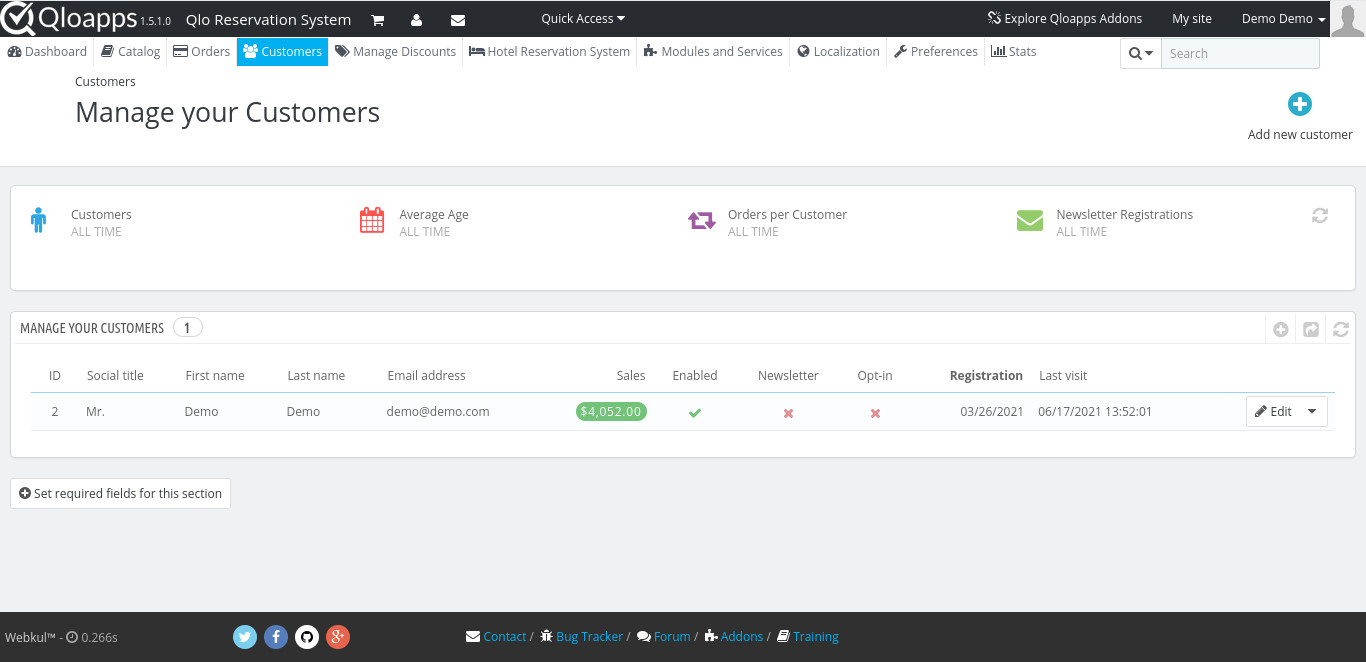
\includegraphics[scale=.5]{imagenes/estado_arte/qlo.png}}
    \caption{Interfaz gráfica de Qlo Hotel \& Booking Reservation}
    \label{fig}
\end{figure}

Esta alternativa podría funcionar aunque con ciertos límites. Entre sus limitaciones algunas como el no poder guardar información personalizada de las personas o que tengan que ser los ``clientes'' los que se asocien a una habitación podría limitar el trabajo de la fundación.

De aplicaciones para gestionar actividades hay más alternativas libres. La mayoría de alternativas ofrecen los que busca la asociación: gestión de actividades, cuentas para residentes, etc. Una de las características que no incluye ninguna de las alternativas libres analizadas es la puntuación y ranking de asistentes, uno de los aspectos diferenciales que la fundación busca perseguir. Algunas de las más interesantes son Agorakit, Gancio o Mobilizon.

En cuanto a alternativas no libres o de pago, es difícil encontrar alternativas asequibles o con planes de precios especializados para organizaciones sin ánimo de lucro. Esto se puede ver como algo normal debido a que está orientado principalmente a un sector comercial.

Finalmente, analizando varias alternativas y diferentes tipos de producto, creo que no existe uno que consiga satisfacer las necesidades de la fundación. Hay varios ``puntos flacos'' que ningun software de los analizados cumple, los cuales formarán parte de las características diferenciales de la alternativa a realizar:

\begin{itemize}
    \item Adaptación total de los datos recogidos a cada una de las personas asociadas con la fundación.
    \item Conexión entre las gestión de las personas de la fundación y su participación en las actividades propuestas por esta.
    \item Gestión de citas de personas, algo que no estaba contemplado en la mayoría de productos debido al estar representadas las personas más como clientes que como residentes.
    \item Búsqueda avanzada en base a las características de los usuarios.
    \item Acceso a estadísticas de la fundación en base a parámetros especificados por ellos mismos.
\end{itemize}

A partir de esto, habiendo analizando y escuchado las preferencias de la organización, lo mejor será el desarrollo de una aplicación móvil personalizada para la propia fundación, incluyendo las características deseadas por esta y adaptándola a su flujo de trabajo.